\problemname{Röksignaler}

\begin{figure}[h] 
\begin{center}
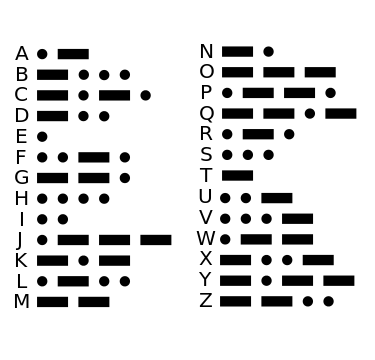
\includegraphics[width=8cm]{morse.png}
\caption{Morsealfabetet}
\end{center} 
\end{figure}

Din kompis är ute på en polarexpedition, och för att hålla kontakten skickar hon röksignaler kodade med morse. Du tycker det är jobbigt att lära dig morsealfabetet utantill, och vill därför skriva ett program som översätter signalen åt dig. Indata är en sträng av ettor och nollor, där en sekvens av ettor motsvarar ett rökmoln. Rökmoln motsvarar streck och prickar, och tomrum motsvarar pauser mellan streck och punkter, bokstäver och mellanslag.

\section*{Input}
De första $26$ raderna innehåller en tabell över morsekoden för alla bokstäver.
Varje sådan rad innehåller en stor bokstav (A-Z), ett mellanslag, och sedan morsekodningen för den bokstaven.

Efter tabellen följer en rad med två olika heltal: $S$ och $P$.
$S$ är antalet ettor som utgör ett streck, och $P$ är antalet ettor som utgör en punkt.

Därefter kommer en rad med tre olika heltal: $T$, $B$ och $M$.
$T$ nollor utgör en paus mellan punkt och streck, $B$ nollor signalerar ny bokstav och $M$ nollor är ett mellanslag.

Till sist kommer en rad som innehåller talet $N$, följt av en $N$ bokstäver lång sträng av ettor och nollor.

\section*{Output}
Din program ska skriva ut en rad som innehåller det avkodade meddelandet.

\section*{Poängsättning}
Din lösning kommer att testas på en mängd testfallsgrupper. För att få poäng för en grupp
så måste du klara alla testfall i gruppen.
\begin{tabular}{| l | l | l | l |}
\hline
Grupp & Poängvärde & Gränser & Övrigt \\ \hline
1     & 19         &  $S = 2, P = 1, T = 1, B = 2$, $1 \le N \le 100$  & Inga mellanslag förekommer\\ \hline
2     & 39         &  $1 \le S, P, T, B, M \le 10$, $1 \le N \le 1000$ & Inga mellanslag förekommer \\ \hline
3     & 25         &  $1 \le S, P, T, B, M \le 100$, $1 \le N \le 1000$    & \\ \hline
4     & 17        &  $1 \le S, P, T, B, M \le 1000$, $1 \le N \le 100000$  & \\ \hline
\end{tabular}
